\documentclass{ctexart}
\usepackage{amsmath}
\usepackage{float}
\usepackage{amssymb}
\usepackage{graphicx}
\usepackage{gbt7714}
\usepackage{pifont}
\usepackage{wrapfig}
\ctexset{
    % 修改 section。
    section={   
        name={,、},
        number={\chinese{section}}
    }
}

\title{光的衍射现象的观察和测量}
\author{陆知辰-10225301478}
\date{\today}
\graphicspath{{figure/}}

\begin{document}

\begin{titlepage}
  \centering
  % 插入图片
  
\includegraphics[width=0.5\textwidth]{ecnu.png}
  
  % 空行用于调整标题位置
  \vspace*{\baselineskip}
  
  % 标题
  \Huge\textbf{物\quad 理\quad 实\quad 验 \quad (二)}
  % 空行用于调整标题和其他信息之间的间距
  \vspace*{0.3\baselineskip}
  
  % 具体实验名称
  \huge 光的衍射现象的观察和测量
  
  % 空行用于调整时间和其他信息之间的间距
  \vspace*{2\baselineskip}
  
  % 时间
  \large 时间:\today
  
  % 空行用于调整时间和其他信息之间的间距
  \vspace*{\baselineskip}
  
  % 创作人
  \large 创作人:陆知辰
  
  % 空行用于调整创作人和学号之间的间距
  \vspace*{\baselineskip}
  
  % 学号
  \large 学号:10225301478
  
\end{titlepage}
\newpage
\tableofcontents
\newpage
\section{实验摘要}
  \subsection{实验概要}
  光的波动性可以通过光的衍射和光的干涉进行证明。光的衍射现象时光的波动性的一种体现。
  衍射就是指当一个波动遇到某种障碍物的时候,这种波动会偏离其原来直线传播的方向。
  通过研究光的衍射能够更好的了解光的本质,同时,光的衍射现象的研究也是近代光学技术的实验基础。

  \subsection{实验目的}
  1.\quad 掌握夫琅和费衍射实验光路的搭建方法

  2.\quad 观察单缝、光栅等的夫琅和费衍射图像,加深对光的衍射理论的理解

  3.\quad 利用衍射图像计算单缝宽度、光栅常量、激光波长等

% \begin{figure}[H]
%   \begin{minipage}[H]{0.4\textwidth}\label{rlcdianlu}
%   \centering
%   \caption{RLC电路}
%   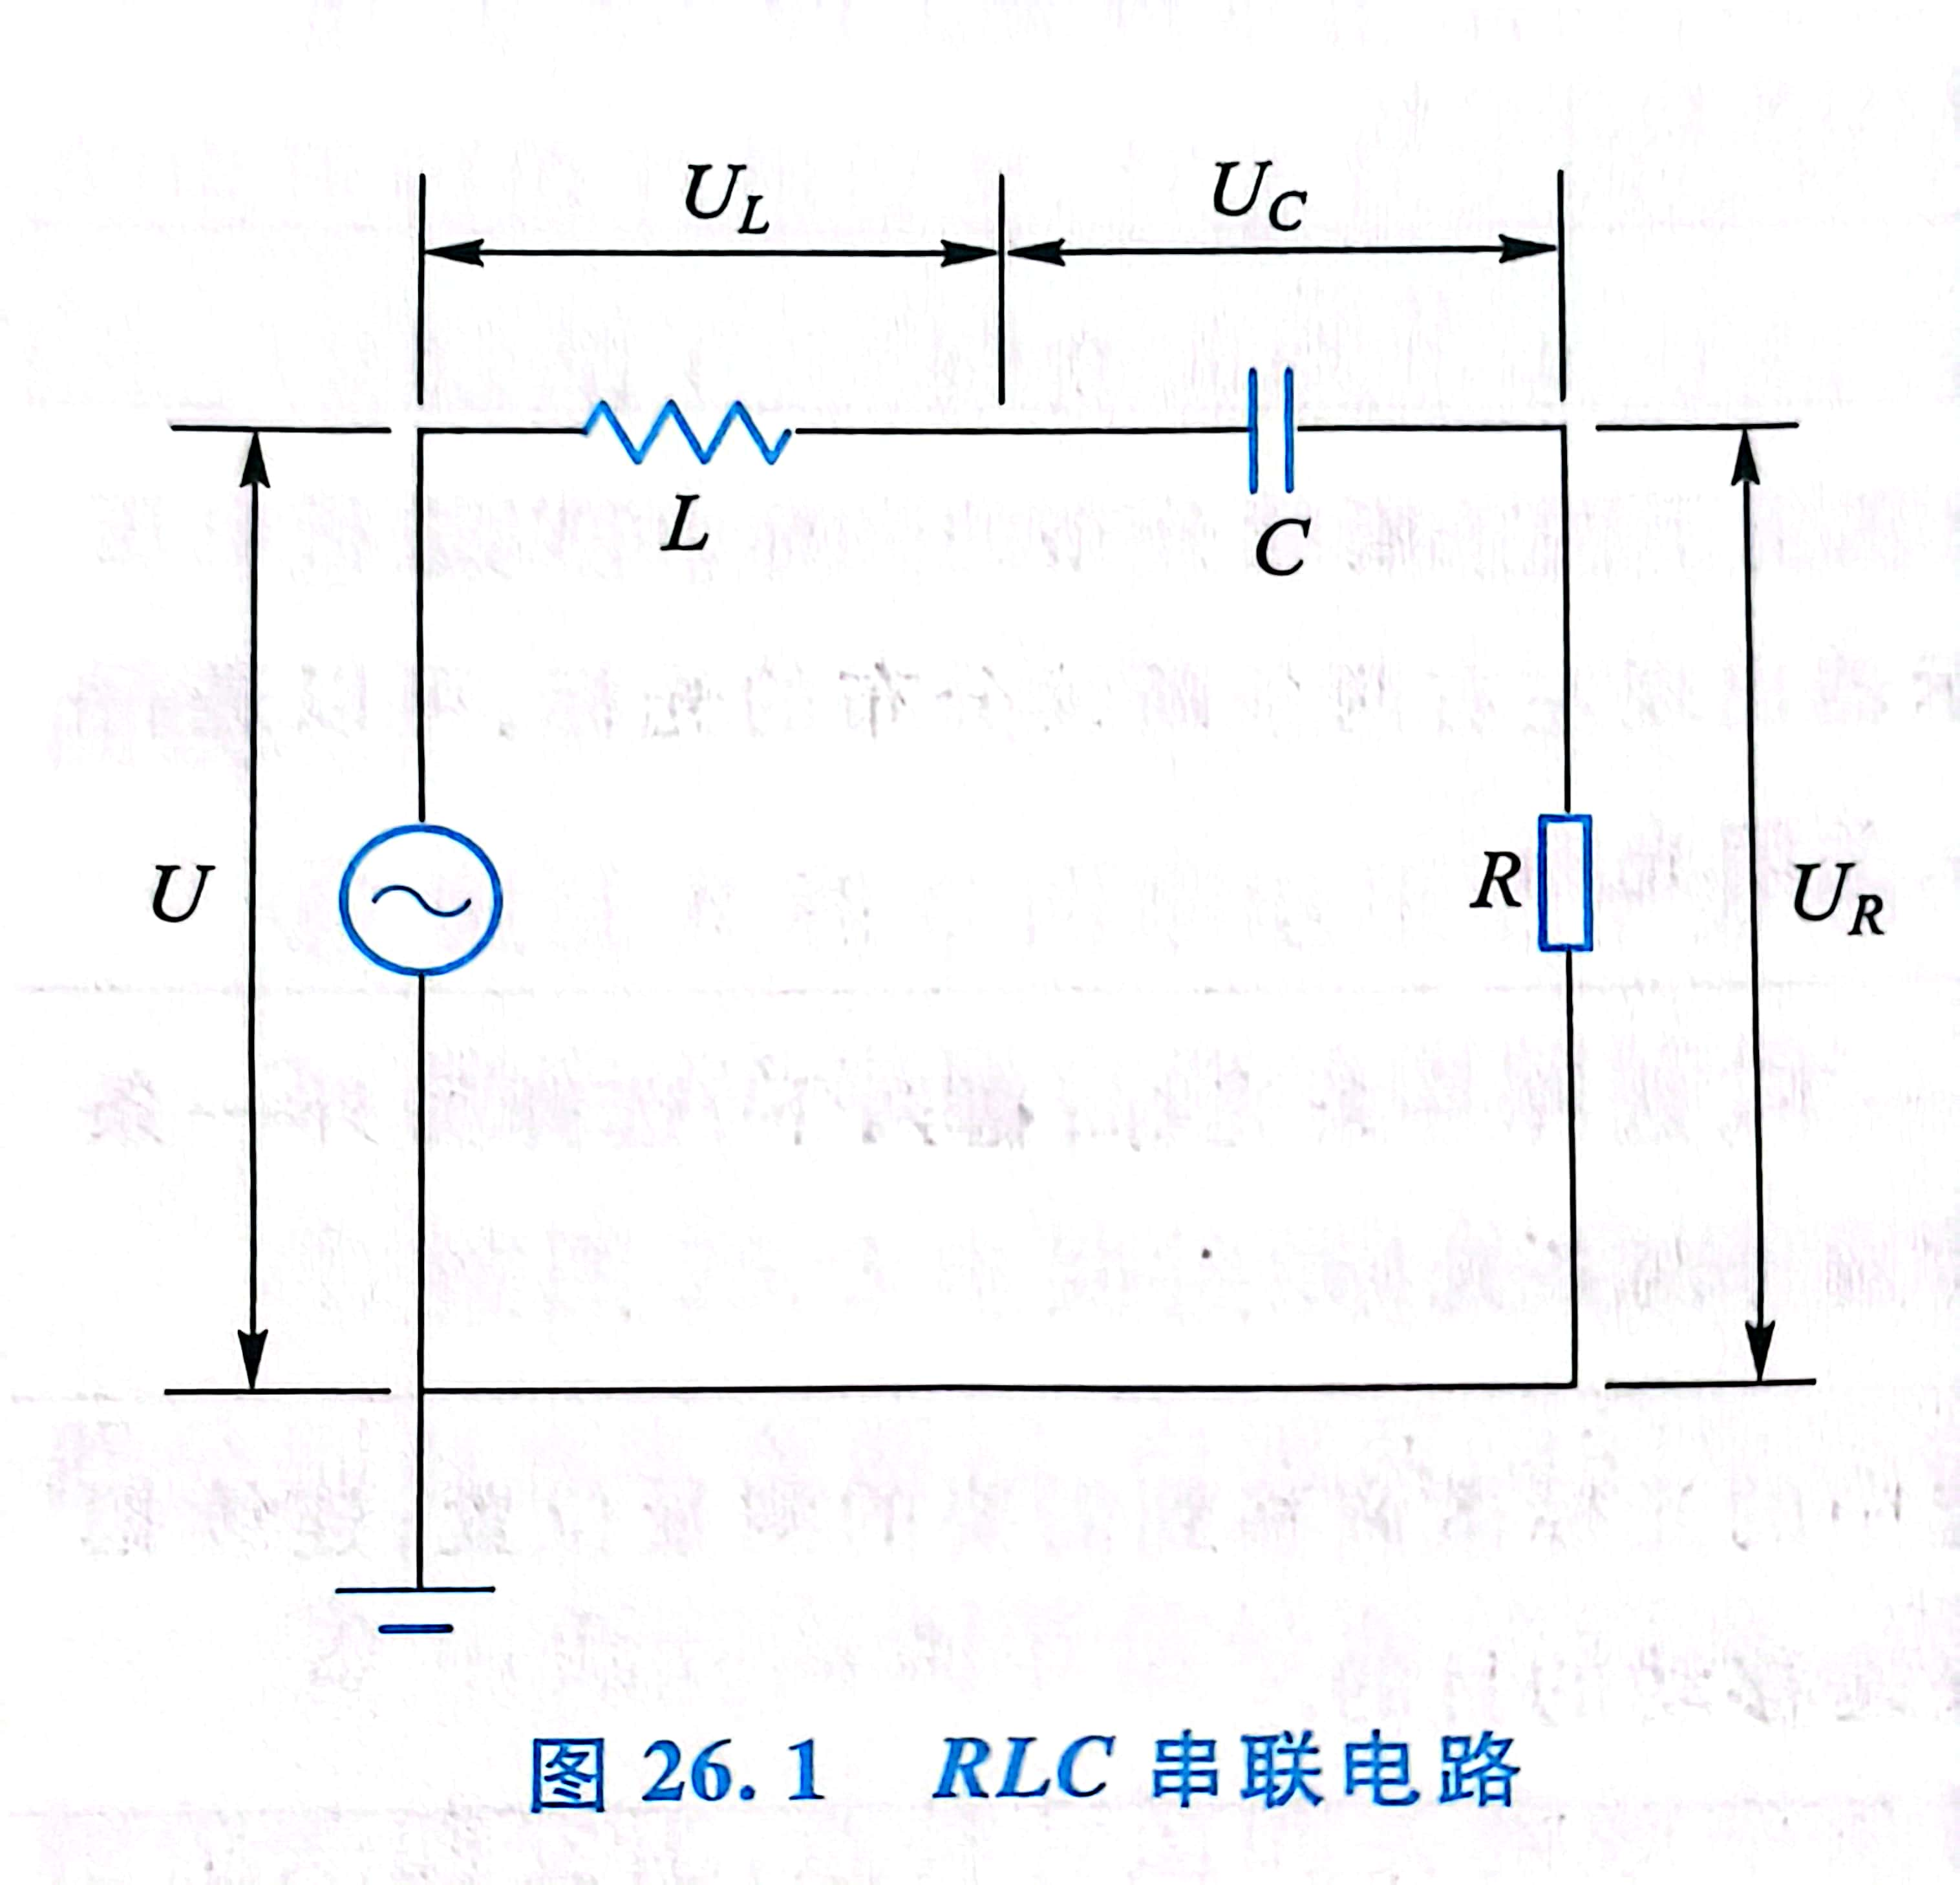
\includegraphics[width=\textwidth]{RLCdianlu.jpg}
%   \end{minipage}
%   \hfill
%   \begin{minipage}[H]{0.4\textwidth}\label{rlcwentaitexing}
%   \centering
%   \caption{RLC稳态特性}
%   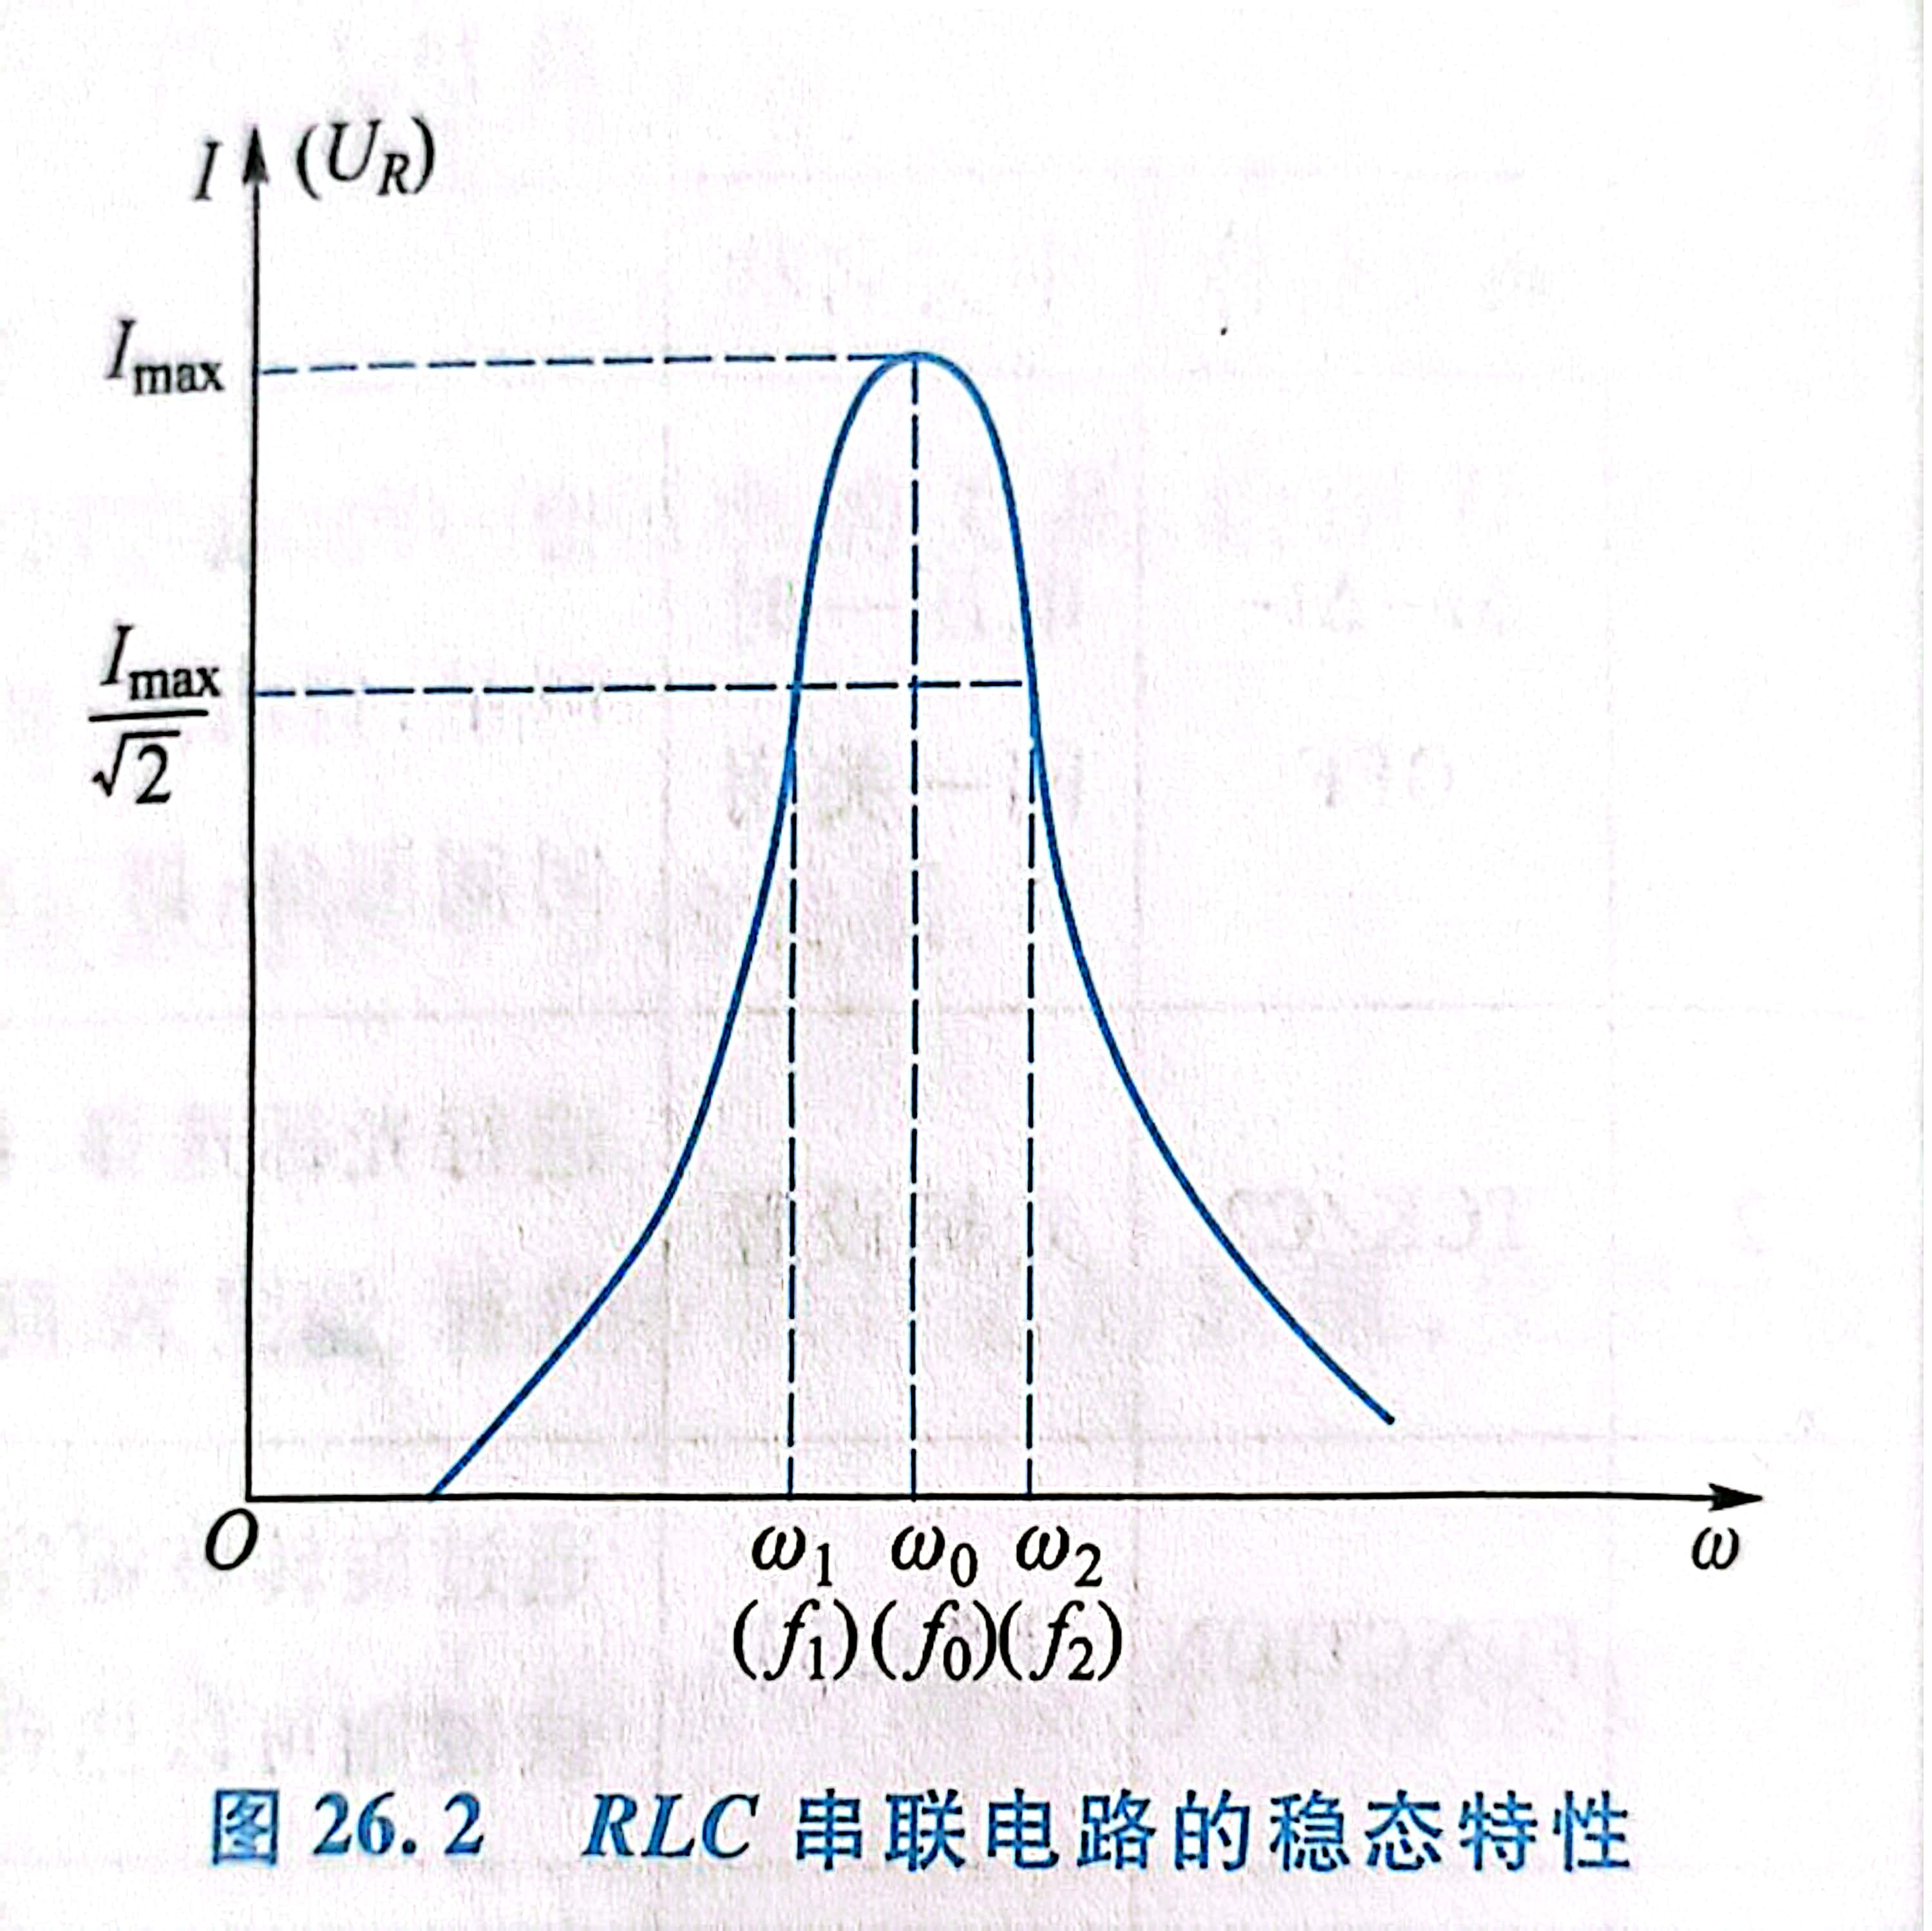
\includegraphics[width=\textwidth]{RLCwentaitexing.jpg}
%   \end{minipage}
% \end{figure}

\section{实验原理}
  \subsection{夫琅和费衍射}
  光在传播的时候遇到障碍物的时候,在实验中也就是衍射元件的时候,能够让绕过障碍物的边缘前进继续传播,
  这种光的偏离直线传播的现象被称为光的衍射。

  夫琅和费衍射是一种特殊的颜色和,在和狼合肥衍射发生时候,入射到衍射元件上的光线是平行光,衍射图像的观察屏与障碍物的距离为无穷远,
  夫琅和费衍射的标准光路图如\ref{flhfguanglu}所示,图中的光源和观察屏分别位于透镜$L_{1}$和$L_{2}$的焦面上,透镜$L_{1}$后的
  平行光则垂直入射衍射元件。

\begin{figure}[H]
  \centering\label{flhfguanglu}
  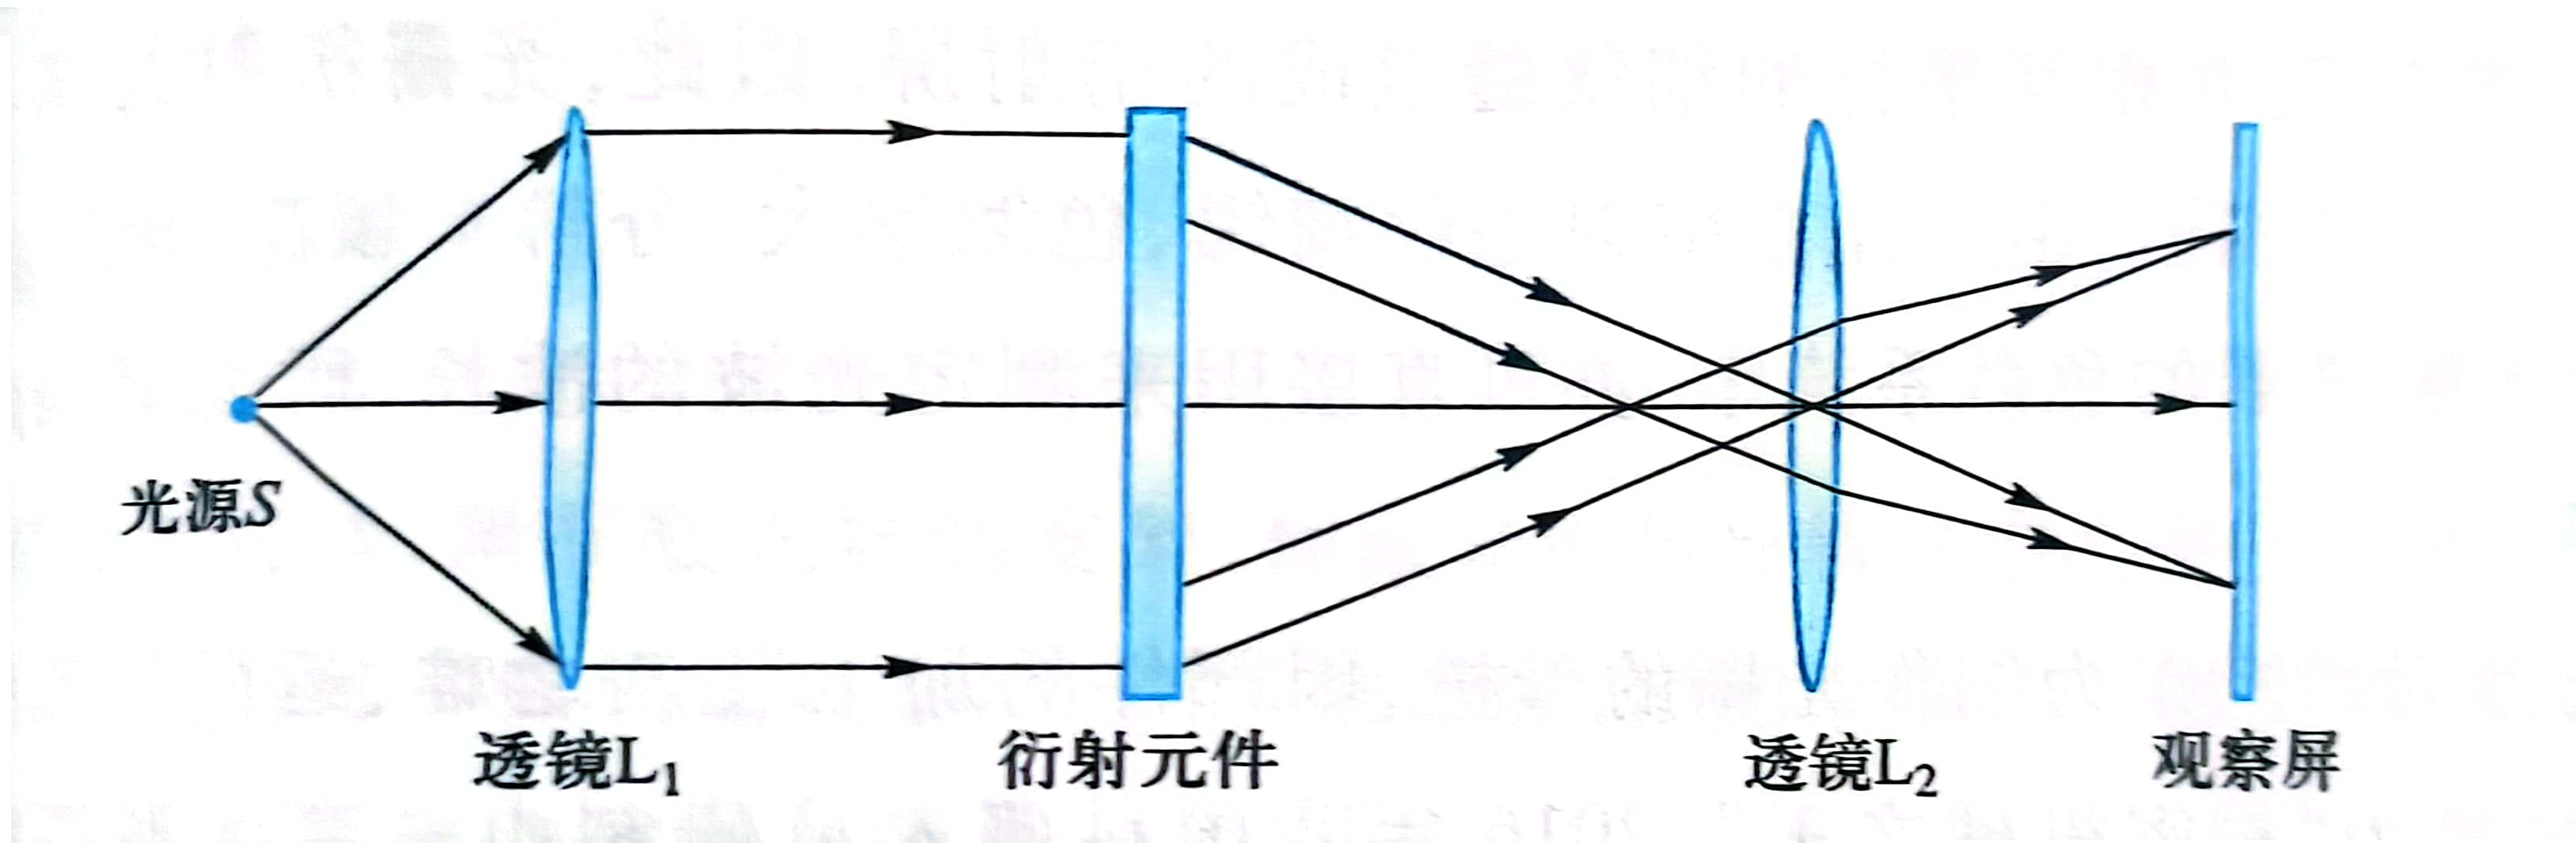
\includegraphics[width=0.9\textwidth,height=0.2\textheight]{flhfguanglu.jpg}
  \caption{夫琅和费光路}
\end{figure}

  激光的平行度较好,光束的发散角较小,可以作为平行光直接豪奢衍射元件,在观察屏和衍射元件的距离
  足够远的条件下,亦可忽略透镜$L_{2}$,此时观察屏与衍射元件之间的距离z满足式\ref{yuanjvli}
  \begin{equation}\label{yuanjvli}
    z>>\frac{\rho^{2}}{\lambda}
  \end{equation}

  其中,$\rho$为衍射孔径的一半,而$\lambda$是入射光的波长。

  \subsection{单缝衍射}
  \begin{figure}[H]
    \centering\label{dfguanglu}
    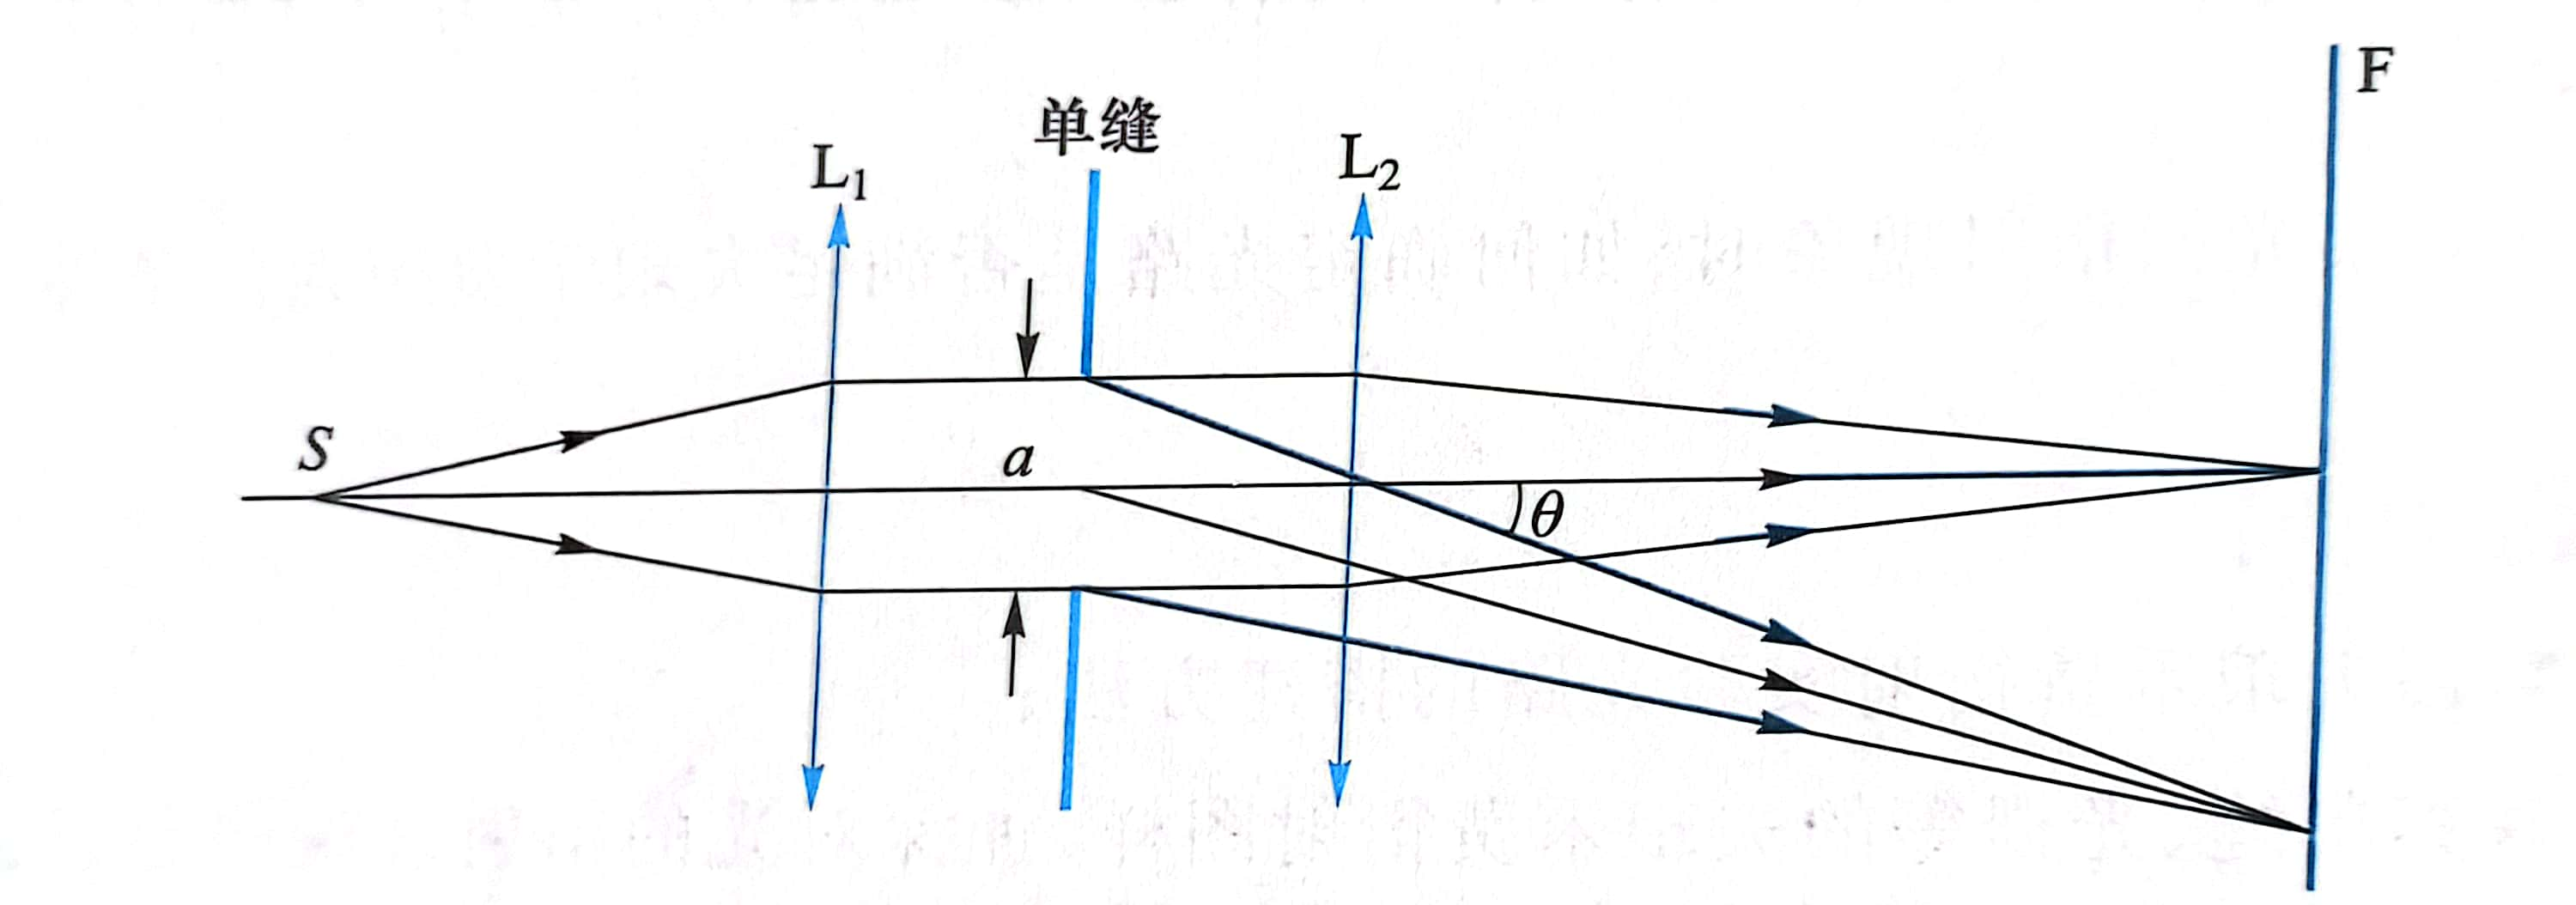
\includegraphics[width=0.9\textwidth,height=0.2\textheight]{dfguanglu.jpg}
    \caption{单缝夫琅和费衍射光路}
  \end{figure}
  如图\ref{dfguanglu}所示,当采用平行光垂直入射单缝的时候,在单缝后方一定区域内将会观察到
  夫琅和费图样,其光强分布满足式\ref{dfflhfgongshi}
  \begin{equation}\label{dfflhfgongshi}
    I_{\theta}=I_{0}\frac{\sin^{2}u}{u^{2}}\quad (u=\frac{\pi a \sin \theta}{\lambda})
  \end{equation}

  其中$I_{\theta}$为衍射光强,$I_{0}$为入射光强,$\theta$为衍射角,$a$为狭缝宽度。
  该式子表明两点:

  1.\quad 当$u=0$时,$I_{\theta}=I_{0}$为最大,称之为主极大。

  2.\quad 当$u=k\pi(k=\pm 1,\pm 2,\pm 3\dots)$,即$a\sin\theta=k\lambda$时,
    $I_{\theta}=0$出现暗条纹,在$\theta$很小的时候,可以使用$\theta$来代替$\sin\theta$,
    因此,暗条纹出现在$\theta=\frac{k\lambda}{a}$处。

  实验上通过测量暗纹的间距可以获得狭缝宽度。

  \subsection{光栅衍射}
  光栅是一种常用的光学色散元件,在结构上具有空间周期性,
  它好似一块由大量等宽、等间距并相互平行的细狭缝组成的衍射屏.因此,
  光栅衍射的基本原理与多缝衍射原理相似.由于光栅衍射条纹细锐、色散率大、分辨本领高,
  因而它通常用在各种光谱仪器的色散系统中,亦可直接用来测定光波的波长,研究谱线的结构和强度等.
  光栅刻划机作为制作光栅的母机,因部件的加工装调之难、运行保障环境要求之高,
  被誉为“精密机械之王”.2016年我国科研人员研制出一套大型高精度光栅刻划系统,
  并成功制作出目前世界上最大面积(400mmx500mm)的中阶梯光栅,打破了我国大型光学系统、
  远程探测与识别等大科学装置以及国家战略高技术领域所需要的高精度大尺寸光栅受制于人的局面。

  \begin{figure}[H]
    \centering\label{gsguanglu}
    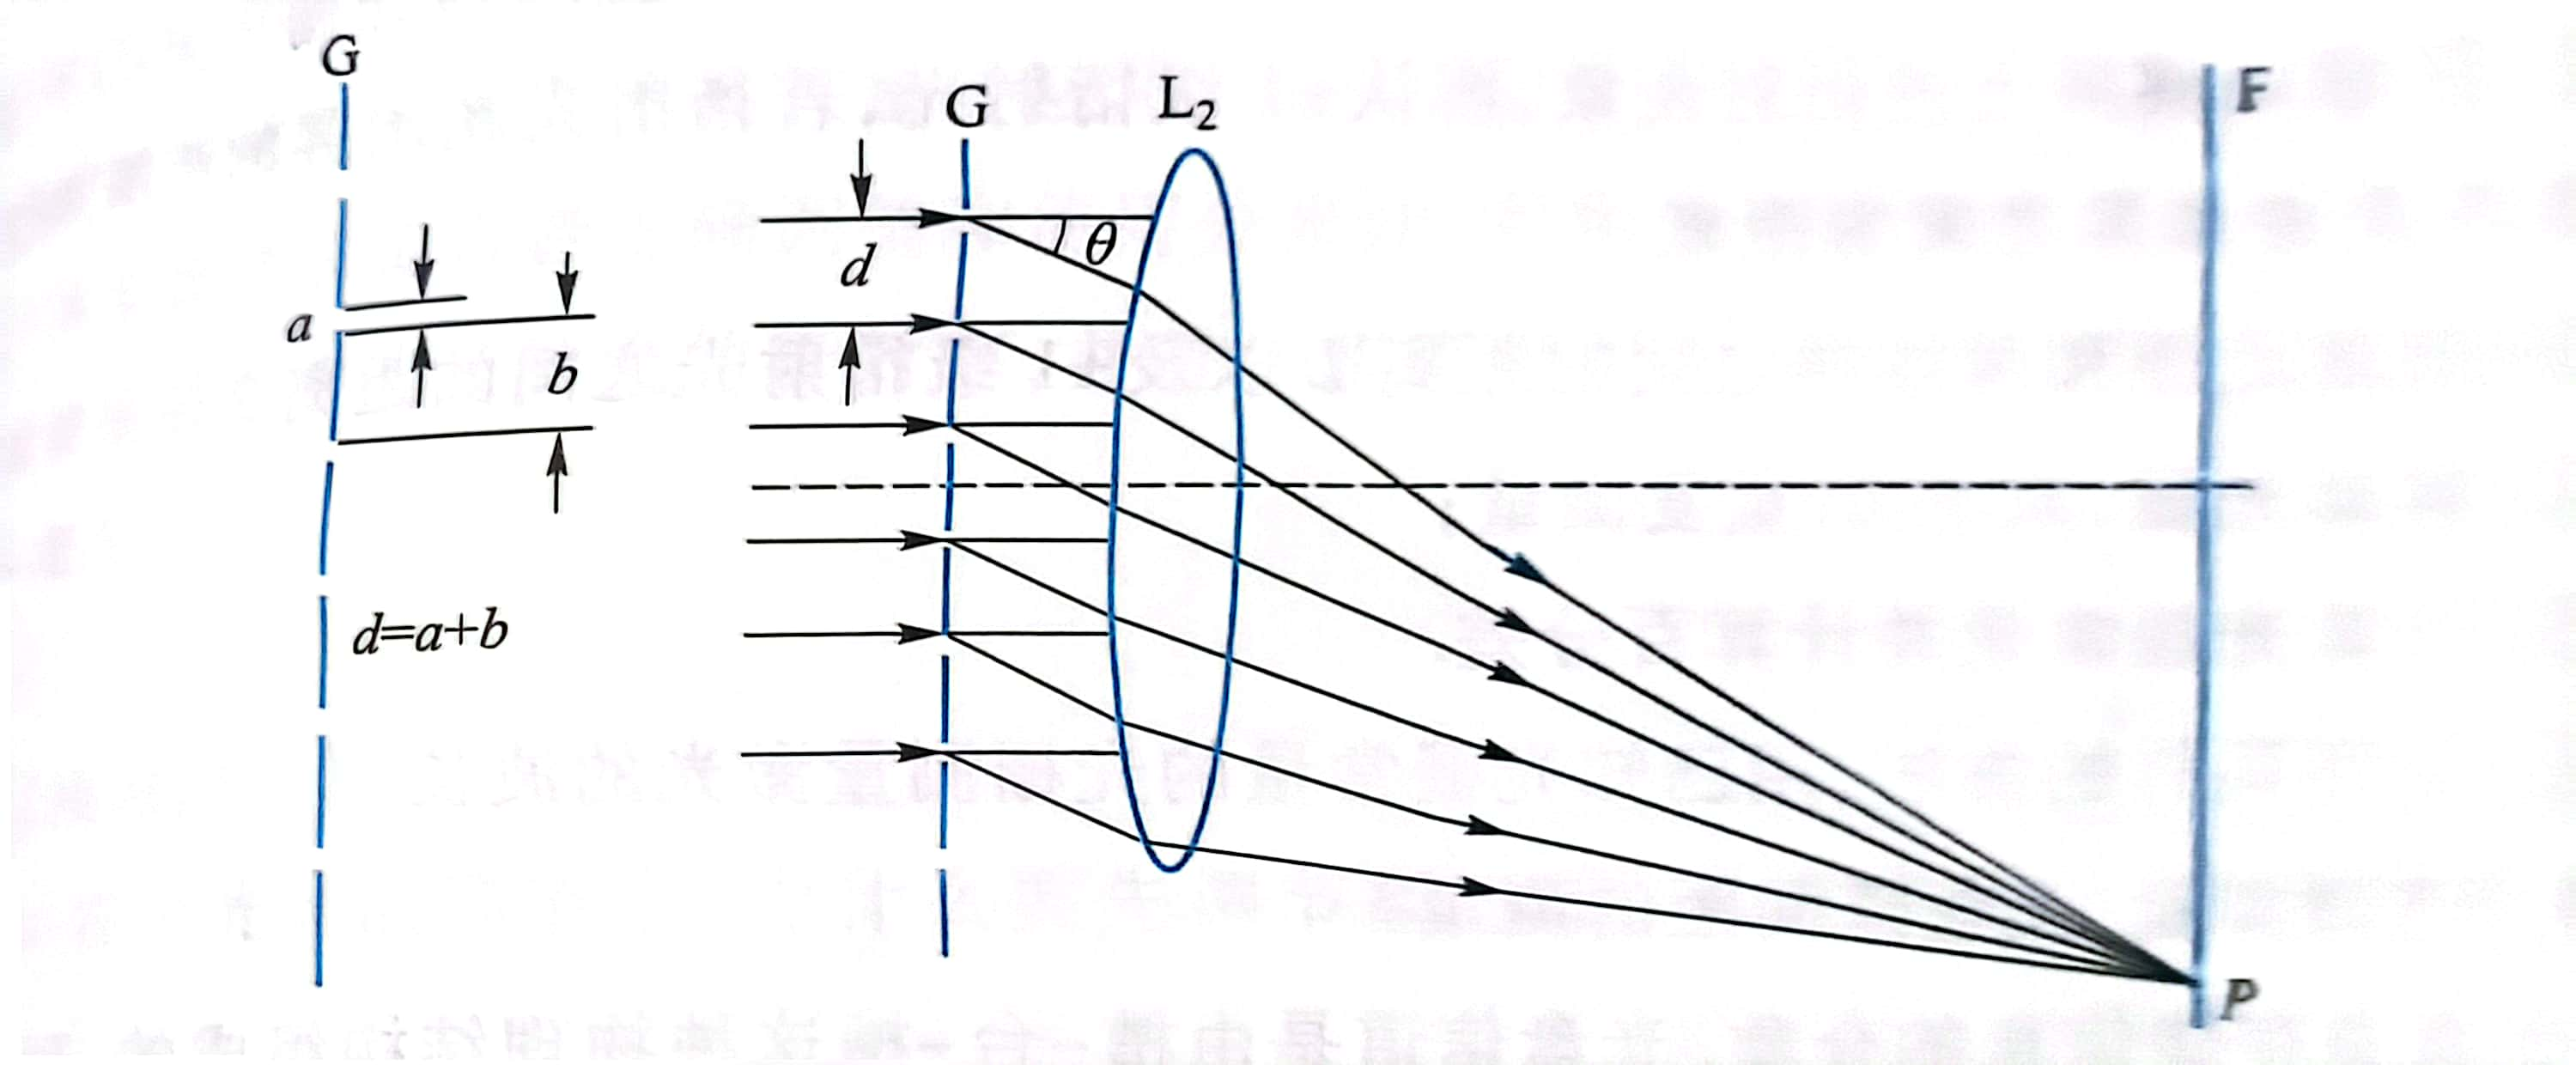
\includegraphics[width=0.9\textwidth,height=0.2\textheight]{gsguanglu.jpg}
    \caption{光栅衍射光路示意图}
  \end{figure}

  光栅衍射光路示意图如图\ref{gsguanglu}所示,G为光栅,它由N条宽度为a的透光缝组成,相邻狭缝间
  不透光的部分宽度为b,平行光垂直照射在光栅G上,在观察屏上P处产生亮纹的条件如式\ref{guangshantaojian}
  \begin{equation}\label{guangshantaojian}
    d\sin \theta = k\lambda
  \end{equation}

  上式即光栅方程,式中$\theta$为衍射角,入是所用光源的波长,
  k是光谱的级次$(k=0,\pm 1,\pm 2,…)$,d=a+b是所用光栅的光栅常量,
  衍射角$\theta=0$时,级次k=0,任何波长都满足在该处为极大的条件,所以,
  $\theta=0$处出现中央亮纹.对于k的其他数值,符号"$\pm$"表示两组光谱,
  它们由中央亮纹向左右对称地分布.
  若光栅$\pm 1$级衍射光与0级光之间的夹角足够小$\theta<5^{\circ}$,则有如下方程近似成立:
  \begin{equation}
    d\sin\theta\approx=d\tan\theta=d\frac{x}{L}=\lambda
  \end{equation}
  式中的x为0级光和$\pm 1$级衍射光之间的距离,L是光栅和观察屏之间的距离。

\section{实验装置器材介绍}
单缝、光栅、激光器、光屏、光具座、游标卡尺

\section{实验内容及实验步骤}
  \subsection{光路的调节}
  \ding{172} 打开激光器,调节激光器的支架,使激光束和导轨中心平行传播。

  \ding{173} 在导轨的另一侧放置观察屏,调节观察屏,使光束垂直入射观察屏的中心。

  \subsection{单缝衍射现象的观察及测量}
  \ding{172} 将单缝放人激光器与光屏之间,调节单缝平面,使激光垂直入射,
  并确保单缝与光屏之间的距离足够远。

  \ding{173} 在观察屏上观察单缝衍射现象,测量±1级暗斑之间的间距,计算单缝宽度。

  \ding{174} 选择两个或两个以上不同缝宽的单缝重复以上实验,分析并总结单缝宽度对衍射现象的影响.
  
  \subsection{光栅衍射现象的观察及测量}
  \ding{172} 在激光器和观察屏之间插入光栅,注意使激光束垂直人射光栅平面。

  \ding{173} 仔细观察屏上的衍射现象,辨认$\pm$1级衍射光。
  若衍射光超出屏的范围,则应适当减小光栅和屏之间的距离。

  \ding{174} 测量光栅和观察屏之间的距离L以及$\pm$1级衍射光之间的距离2x。

  \ding{175} 移动光栅,减小L,重复测量。

  \ding{176} 计算光栅常量并计算百分差。

  \ding{177} 采用同样的方法,用已知光栅常量的光栅测量激光的波长。
\newpage

\section{实验原始数据}
\begin{figure}[H]
  \centering
  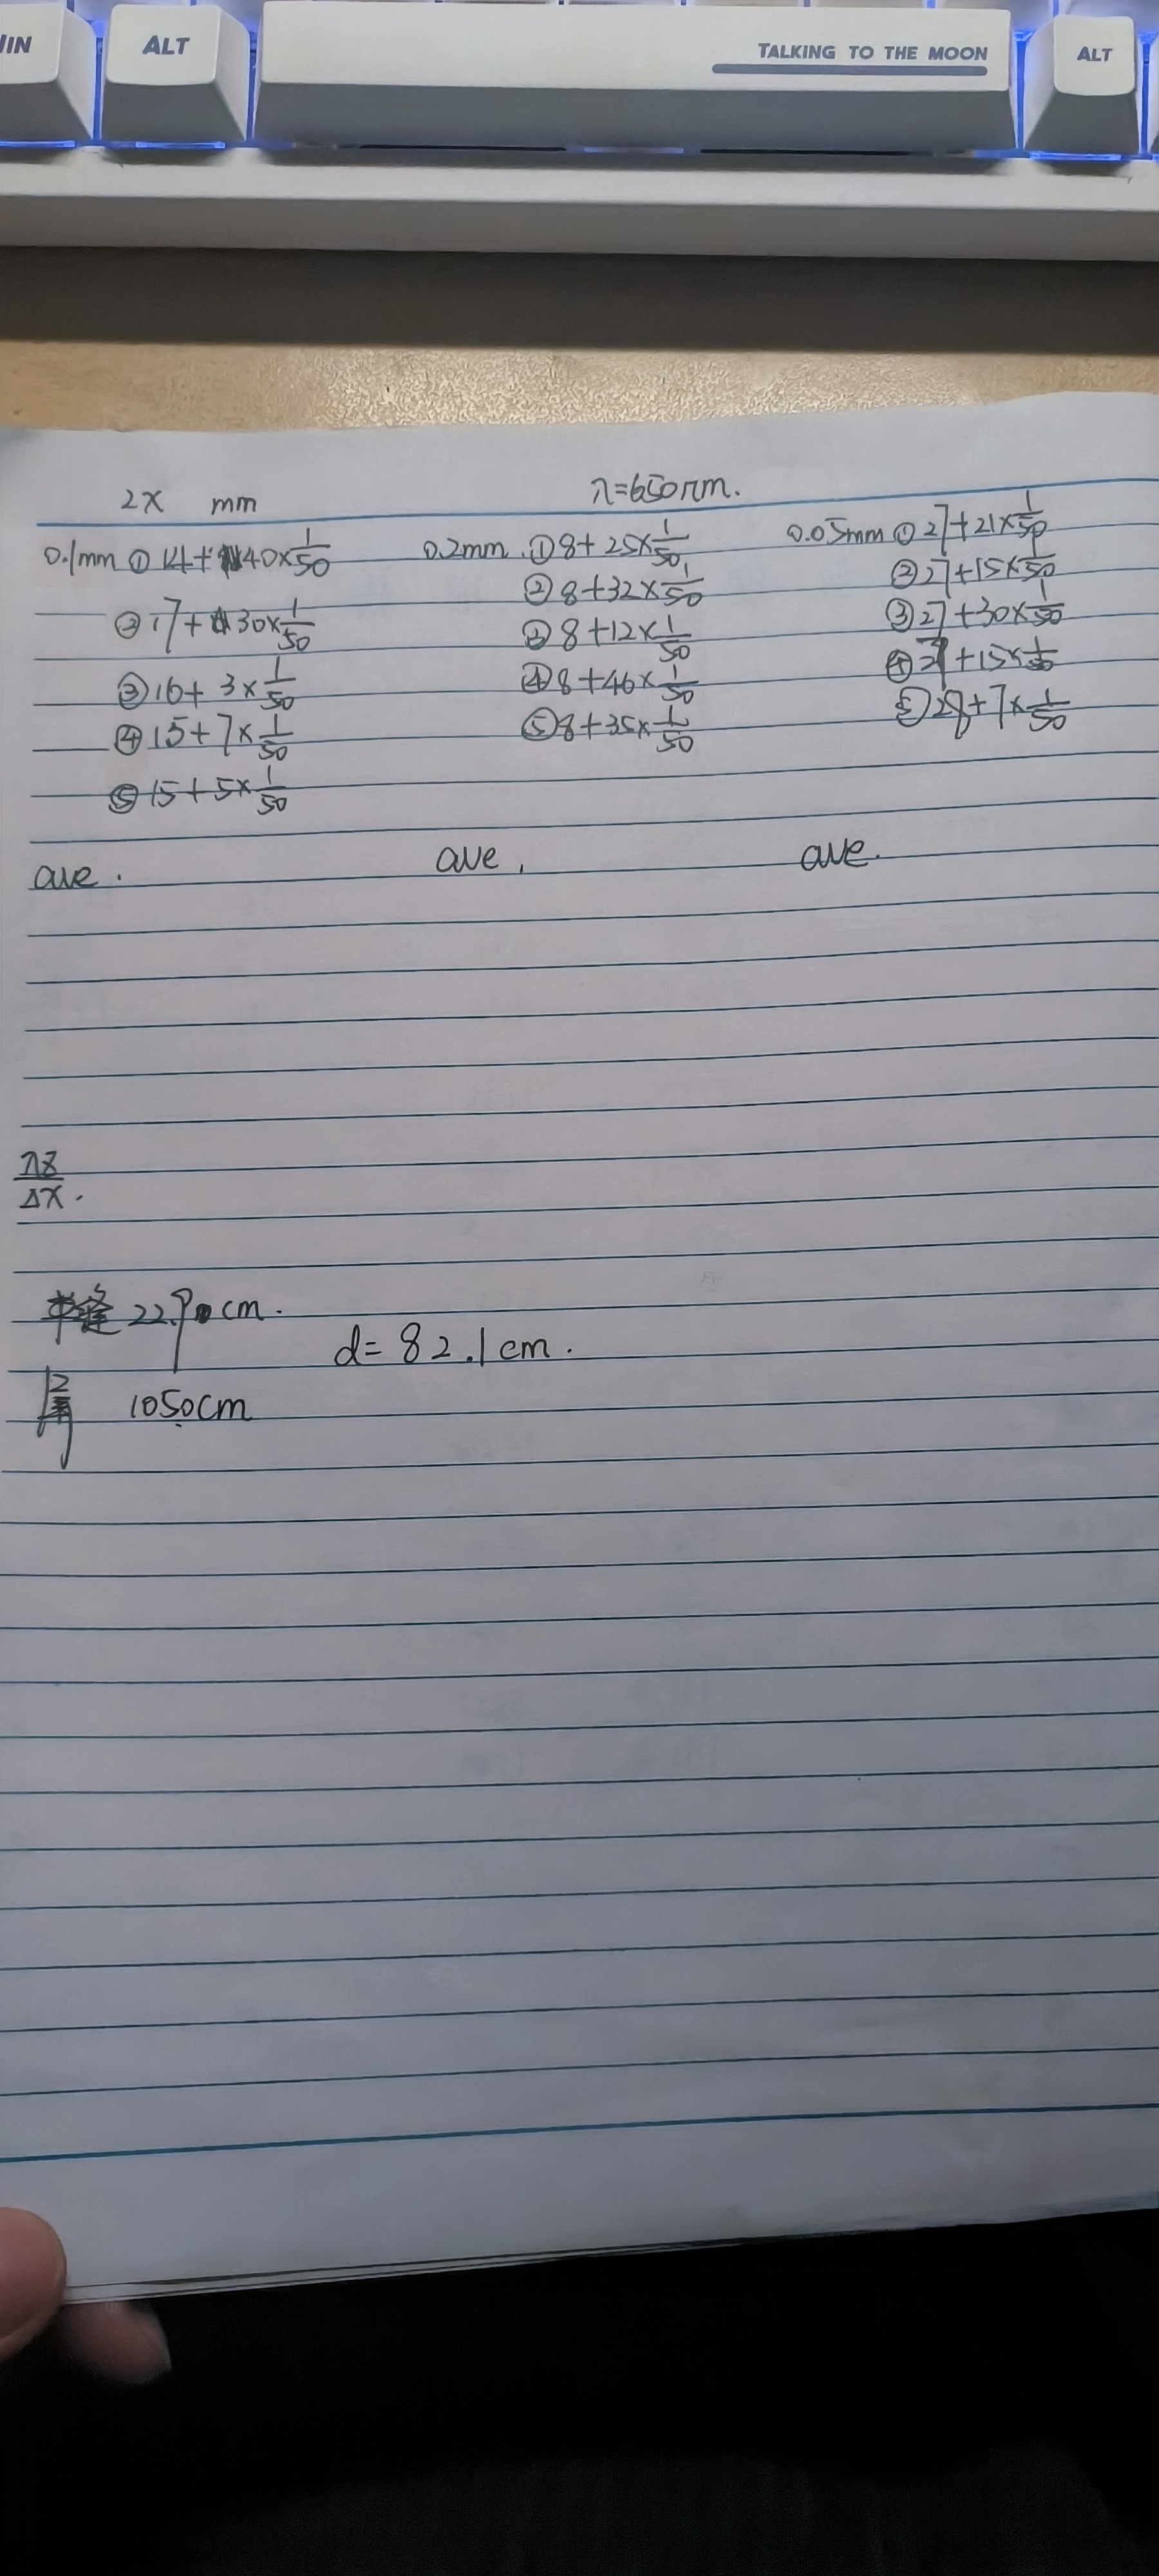
\includegraphics[width=0.9\textwidth,height=0.8\textheight]{yuanshishujv1.jpg}
  \caption{实验原始数据1}
\end{figure}
\newpage

\begin{figure}[H]
  \centering
  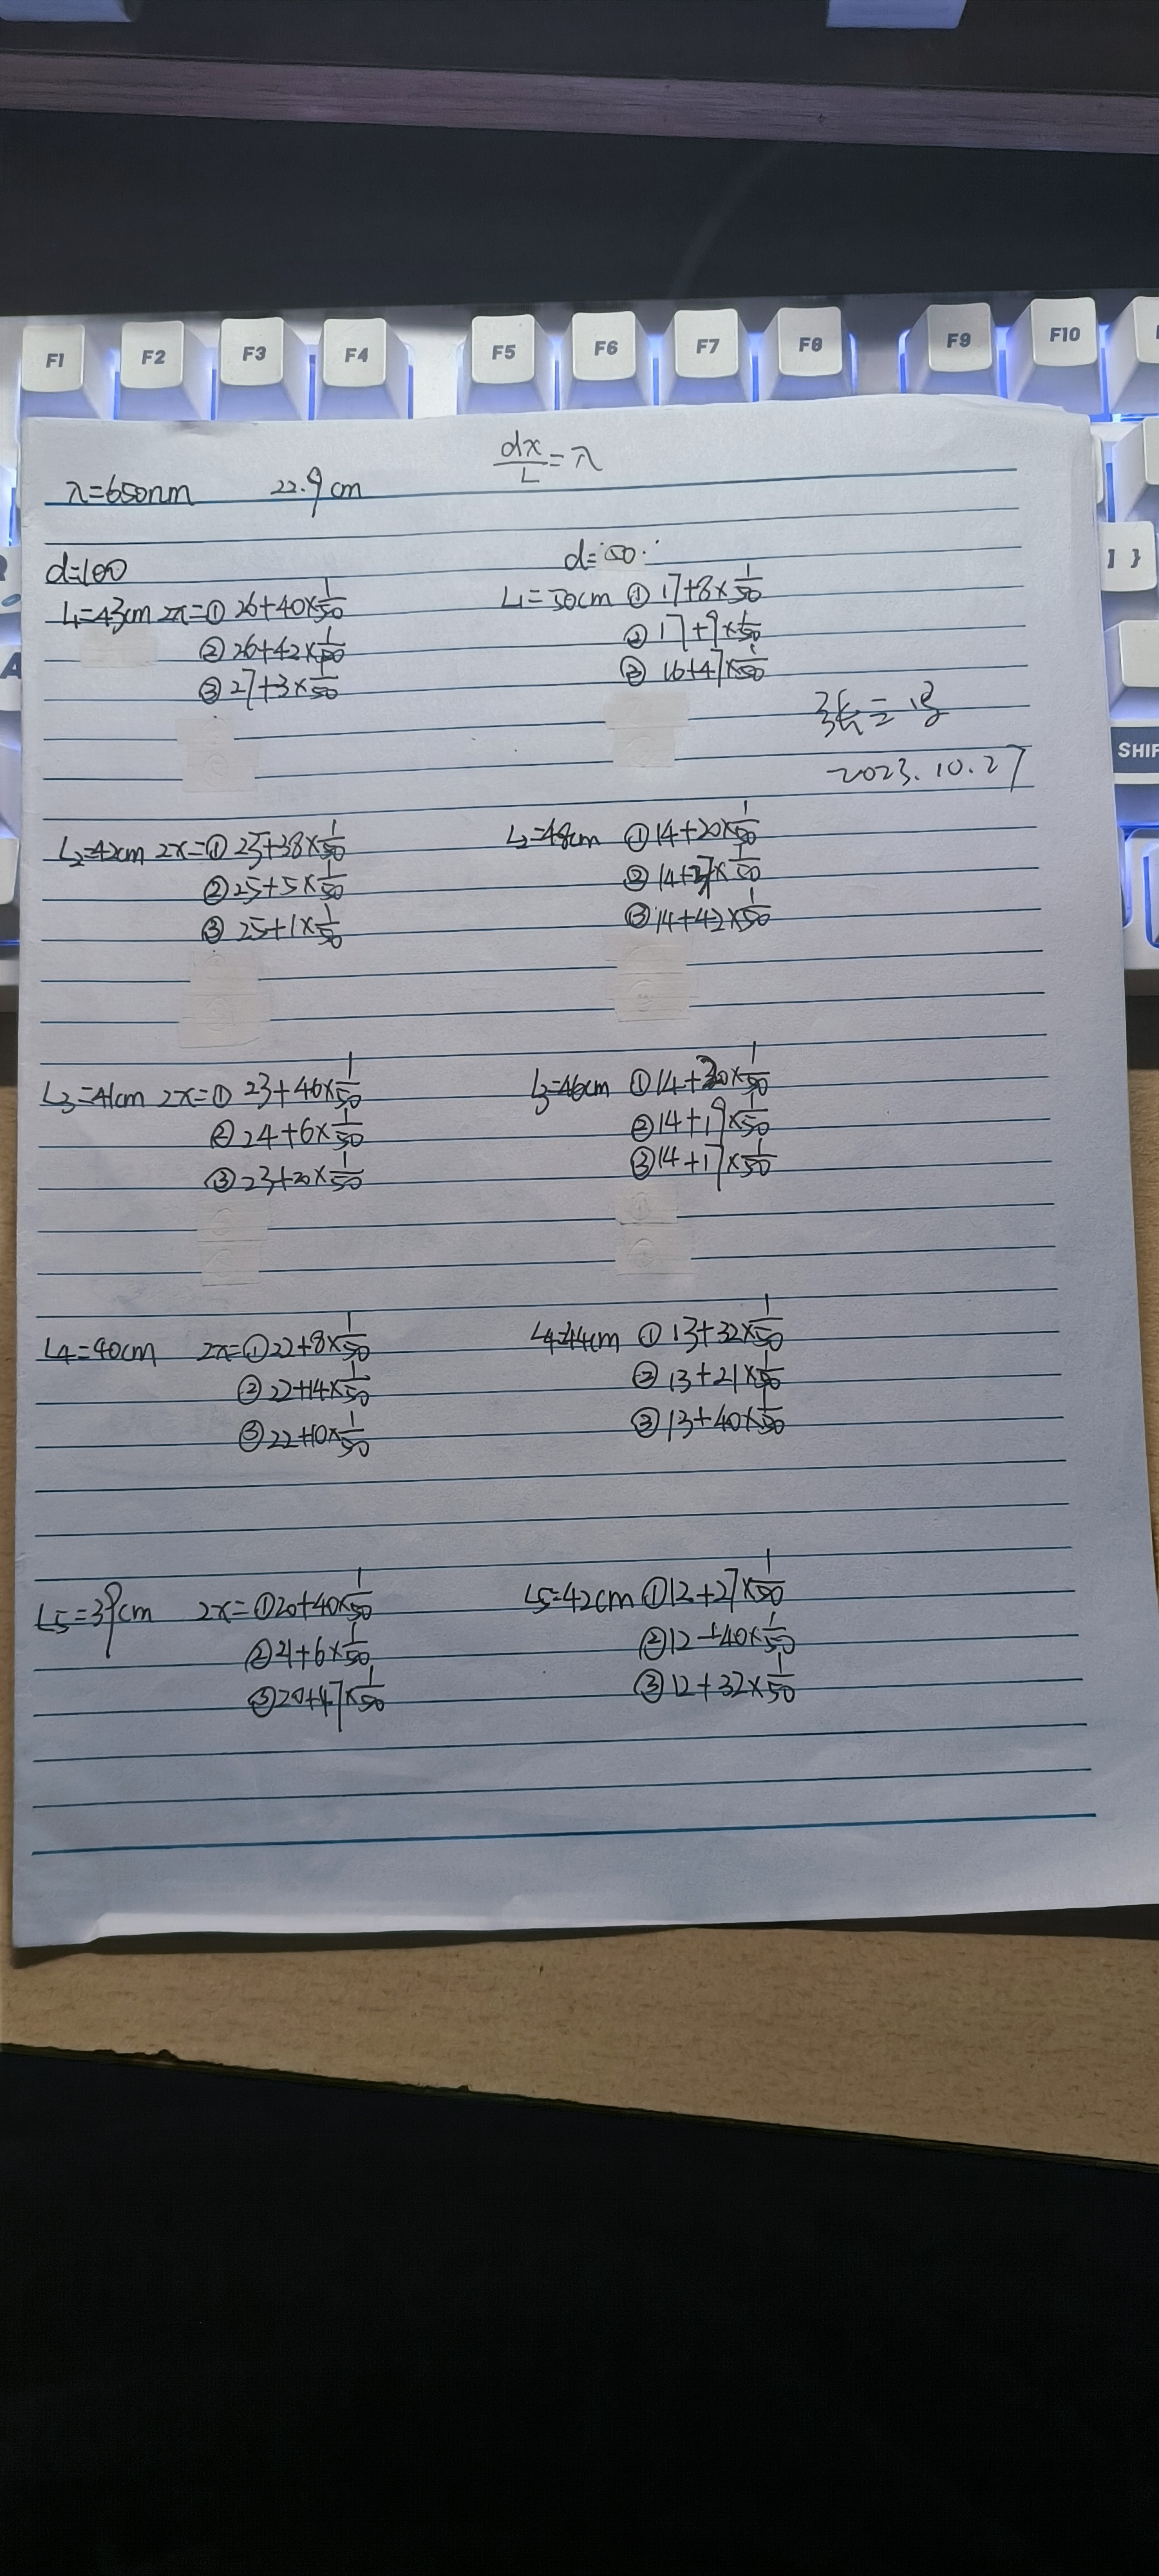
\includegraphics[width=0.9\textwidth,height=0.8\textheight]{yuanshishujv2.jpg}
  \caption{实验原始数据2}
\end{figure}
\newpage

\section{实验数据处理}
  \subsection{单缝衍射现象的观察及测量}
  实验数据处理如图:
  \begin{figure}[H]
    \centering
    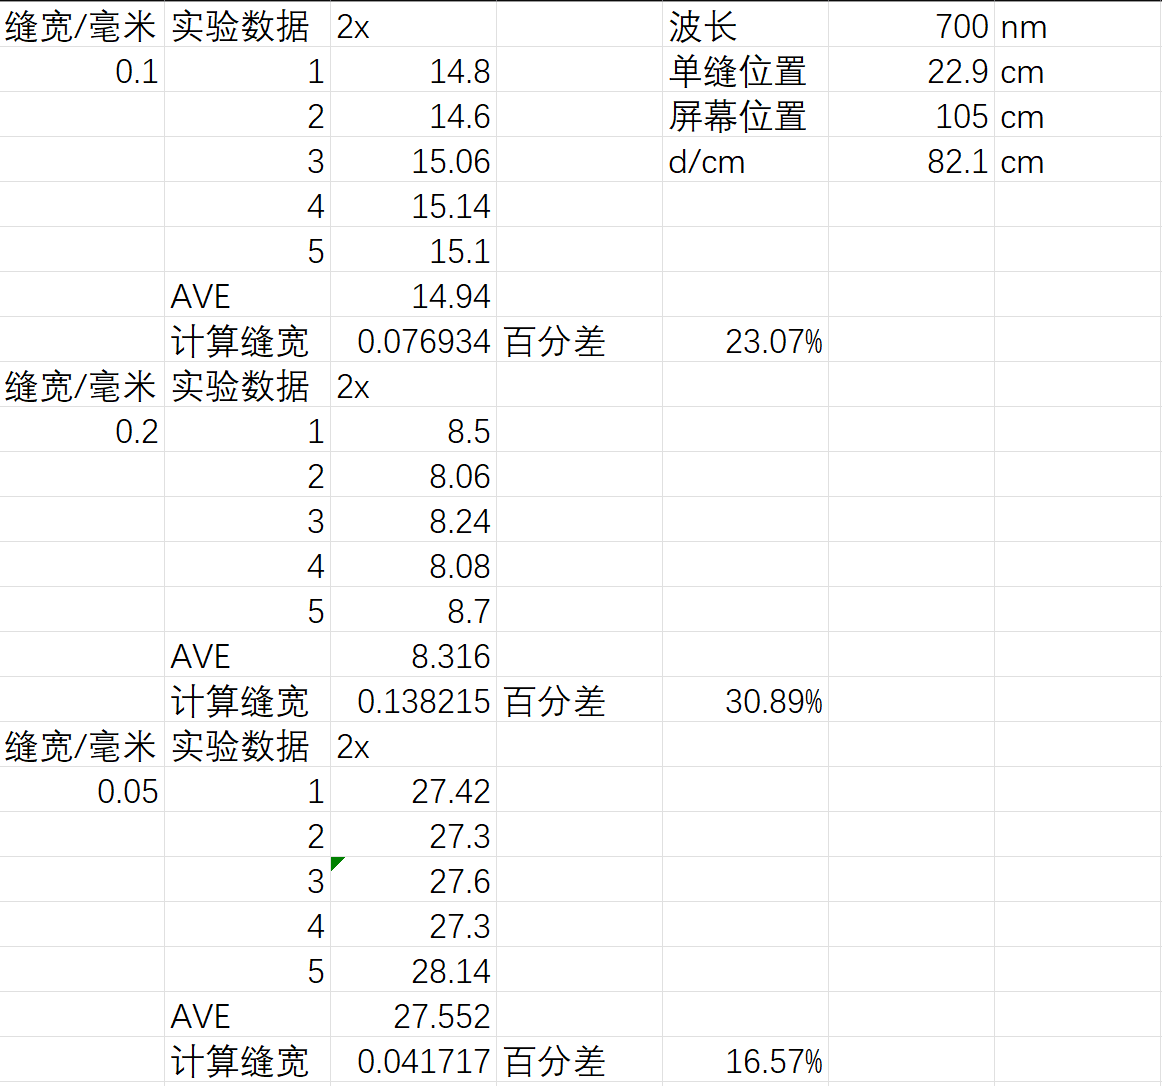
\includegraphics[width=0.9\textwidth,height=0.3\textheight]{danfengshujv.png}
    \caption{单缝衍射现象的观察及测量数据处理}
  \end{figure}

  通过实验结果可以得到在单缝宽度越小的时候,测量结果得到的单缝越接近真实值,数据越准确,百分差越小。
  这也同时说明衍射现象出现在细小缝隙时。

  实验中测得的数据和理论计算得到的数据的百分差较大。
  最终得到的结果误差较大,出现百分差较大的情况,分析误差产生原因:

  1.  测量值可能不够准确,由于器材的误差出现导致实验得到的值不够准确。

  2.  实验中难以确定衍射条纹的边界,每次测量边界都不一样,较为模糊。

  3.  光波波长使用650nm,可能和实际波长有误差。

  \subsection{光栅衍射现象的观察及测量}
  实验数据处理如图:
  \begin{figure}[H]
    \centering
    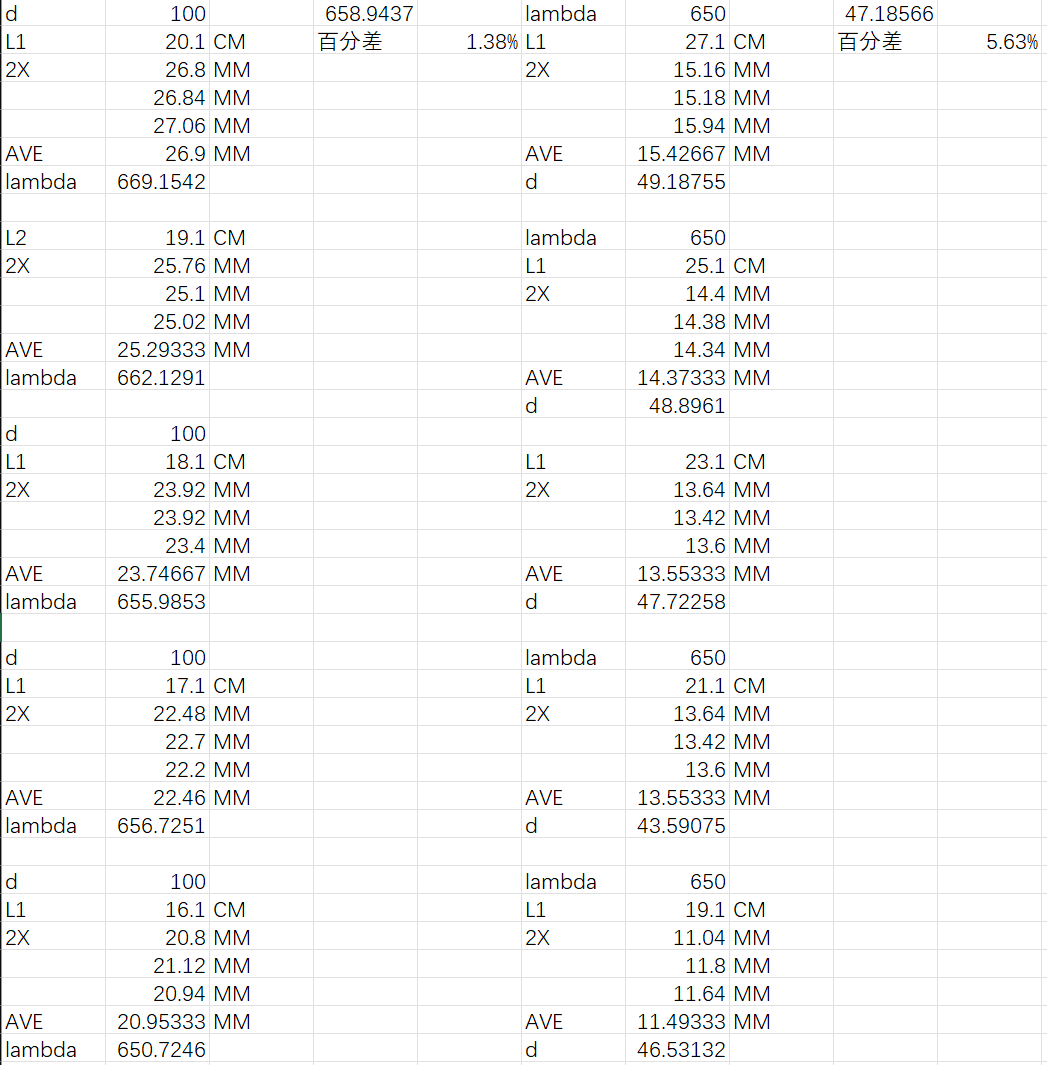
\includegraphics[width=0.7\textwidth,height=0.8\textheight]{guangshanshujv.png}
    \caption{光栅衍射现象的观察及测量数据处理}
  \end{figure}

  数据中左侧一列为已知光栅常量通过实验测量一级条纹间距得到波长数据。

  数据中右侧一列为已知波长通过实验测量一级条纹间距得到光栅常量数据。

  两者百分差前者较小,后者较大。
  最终得到的结果误差较大,出现百分差较大的情况,分析误差产生原因:

  1.  测量值可能不够准确,由于器材的误差出现导致实验得到的值不够准确。

  2.  实验中难以确定衍射条纹的边界,每次测量边界都不一样,较为模糊。

  3.  光波波长使用650nm,可能和实际波长有误差。

\section{思考题}
  \subsection{思考题一}
  实现夫琅禾费衍射的条件是光源和白屏离衍射孔(或衍射缝)的距离为无限远,因为夫琅禾费衍射是远场衍射。

  实验中通过光屏接住衍射图像进行观察。
  \subsection{思考题二}
  使用白光进行试验将会看到彩色的衍射条纹,中央两条纹为白色。

  \subsection{思考题三}
  衍射图形会发生偏移。
  光栅平面和入射光本来也就不用垂直的。光栅的公式里也有入射角这么一项。
  而一般的光谱仪在改变波长范围时都是旋转光栅的。
  衍射条纹会相应地移动一个角度,最终会引入一定误差,因为计算公式中没有将入射角考虑进去。

\section{实验中个人的思考与感想}
  \subsection{对于实验个人观点}
  实验整体还是不难的,但是实验中激光的强度不够导致在单缝衍射现象观察中出现难以分辨边界的情况。
  
  而光栅实验中虽然光强足够,但是还是会出现衍射图像边界不清,导致实验中测量边界的时候很难确定具体
  范围,也非常容易引入误差。

  \subsection{实验中的总结}
  实验中测量量不够准确,但是通过实验依旧能观察到衍射现象,而单缝衍射的结果和光栅衍射的结果并不相同,
  相较于单缝衍射,通过光栅的能量更多,光屏上的现象也更强。
\end{document}
